\documentclass{article}
\usepackage[spanish]{babel}
\usepackage{graphicx} % Required for inserting images
\usepackage{lipsum}
\usepackage[a4paper, total={6in, 8in}]{geometry}
\usepackage{setspace}
\usepackage[utf8]{inputenc}
\usepackage{csquotes}
\usepackage{amssymb,amsmath,amsthm, amsfonts}
\usepackage{array}

\usepackage{hyperref}
\hypersetup{
    colorlinks=true,
    linkcolor=blue,
    filecolor=magenta,      
    urlcolor=cyan,
    pdftitle={Overleaf Example},
    pdfpagemode=FullScreen,
    }
\urlstyle{same}

\usepackage{xcolor}
\usepackage{listings}

\definecolor{mGreen}{rgb}{0,0.6,0}
\definecolor{mGray}{rgb}{0.5,0.5,0.5}
\definecolor{mPurple}{rgb}{0.58,0,0.82}
\definecolor{backgroundColour}{rgb}{0.95,0.95,0.92}

\lstdefinestyle{CStyle}{
    backgroundcolor=\color{backgroundColour},   
    commentstyle=\color{mGreen},
    keywordstyle=\color{magenta},
    numberstyle=\tiny\color{mGray},
    stringstyle=\color{mPurple},
    basicstyle=\footnotesize,
    breakatwhitespace=false,         
    breaklines=true,                 
    captionpos=b,                    
    keepspaces=true,                 
    numbers=left,                    
    numbersep=5pt,                  
    showspaces=false,                
    showstringspaces=false,
    showtabs=false,                  
    tabsize=2,
    language=C
}

\lstset{style=CStyle}


\setlength{\parskip}{2pt}

\spacing{1.3}

\title{Informe Memcached}
\author{Agustín Samper, Agustín Mangona}
\date{Enero 2024}

\begin{document}
\maketitle
\newpage
\tableofcontents
\newpage
\addcontentsline{toc}{section}{Introducción}
\section*{Introducción}
  En este informe detallaremos el funcionamiento de la \textbf{Memcached} solicitada como trabajo practico final de la asignatura Sistemas Operativos 1 (T1018) correspondiente al tercer año de la carrera de Licenciatura en Ciencias de la Computación de la Facultad de Ciencias Exactas, Ingeniería y Agrimensura de la Universidad Nacional de Rosario.
    
  Una memcached es un sistema de memoria caché con pares claves-valor accesible por la red. Separaremos entonces nuestro análisis de esta implementación en tres secciones, primero veremos como se implementa la memoria cache, luego el servidor que permite acceder a ella por la red, y por último veremos la implementación de un cliente que facilita su uso.
\newpage
\section{Implementación de la caché}
\subsection{Estructura principal}
Decidimos implementar la caché usando un array de punteros
a nodos, los cuales en el código son definidos como estructuras
de tipo List. Cuando se quiere insertar un elemento se pasa
la clave, el valor entre otras cosas, se hashea
la clave para obtener el índice del array en dónde insertarla
y se inserta en la lista correspondiente a esa posición
del array. En resúmen la caché funciona como una tabla
hash pero con algunas modificaciones para el desalojo de
elementos. Además el tamaño del array inicial no puede
ser modificado con lo cual la tabla hash no posee un rehash.

Estructura principal de la cache:
\begin{lstlisting}[style=CStyle]
typedef struct _Cache {
  List *listArr; //Array de punteros a estructura de tipo list 
  unsigned size; //Numero de slots para listas
  Evict evict; //Estructura utilizada para el desalojo de elementos ingresados
  pthread_mutex_t* mutex_arr; //Mutexes para las listas
  unsigned size_mutex_arr; //Cantidad de mutexes
  Stats stats; //Estructura que guarda informacion de uso de la cache
}; 
\end{lstlisting}

\subsection{List}

El nodo de la lista está definido de la siguiente manera:

\begin{lstlisting}[style=CStyle]
typedef struct Node {
  char* key;
  char* value;
  uint32_t lenKey;
  uint32_t lenVal; 
  int isBin; // 1 si los valores
             // guardados en el nodo
             // estan en binario,
             // 0 si no
  struct Node* next;
  struct Node* prev;    
  /**
   * Puntero al nodo que apunta a este nodo
   * en la estructura evict  
  */
  NodeEvict evict;
} Node; 
\end{lstlisting}

Decidimos hacer el nodo con puntero al siguiente y al
nodo previo ya que de esta manera es más sencillo y
óptimo para desalojar elemento en la lista 
(se puede hacer en O(1)). Además el resto de operaciones,
como put, get y del también son bastantes eficientes si
la cache no está demasiado sobrecargada.

evict dentro de Node sirve para el desalojo, pero lo
explicaremos más adelante.

Para implementar la caché pensamos en hacer que cada slot
del array apunte a un avl, pero la implementación es más
compleja que la implementación con listas y además no
tiene muchas ventajas, ya que al no haber
muchas colisiones, no tendremos árboles grandes y no le 
sacaremos provecho a las propiedades del avl. Además al
eliminar o desalojar un nodo de la cache, deberíamos
balancear el árbol que contenía el nodo eliminado y por
lo tanto tomará mayor costo computacional que con las
listas.

Otra forma de implementar la caché pudo haber sido usando
una tabla hash como la siguiente 
\href{https://dspace.mit.edu/handle/1721.1/130693}{RobinHood-MIT}
pero también deberíamos hacer más operaciones para reacomodar los
elementos al eliminar o desalojar. Además la implementación
es más compleja que la implementación con listas.

Para implementar la caché decidimos usar listas en cada
slot del array ya que al tener una gran cantidad de
slots no habrá muchas colisiones y por lo tanto no
se tendrán listas con muchos elementos. Además se
espera que se termine la memoria asignada al programa
antes de que empiece a haber muchas
colisiones, de esta manera se empezarán a desalojar
elementos de la cache y no se llegará a tener un alto
factor de carga.

\subsection{Concurrencia}
\begin{figure}[ht]    
    \centering
    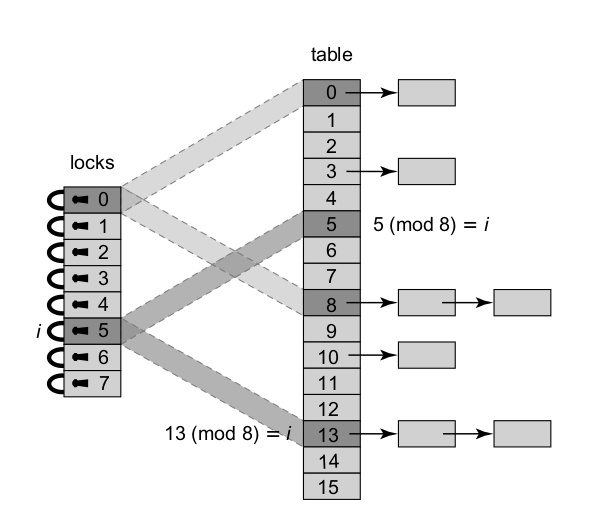
\includegraphics[width=0.7\linewidth]{concurrenciaHT.png}
    \caption{locks in hashtable}
    \label{}
\end{figure}

Para manejar la concurrencia en la tablahash nos basamos en el libro
the art of multiprocessor programming de Maurice Herlihy y Nir Shavit
en el cual, se habla sobre striped hash set y se muestra la figura 1.
Para sincronizar los procesos creamos la misma cantidad de mutexes
que la cantidad de procesadores que tenga la pc que esté corriendo
el programa y particionamos el conjunto de slots del array de listas
de la siguiente manera:

Sea $listaArr$ el array de listas tal que $listArr$ tiene $n$ slots y sea $mutexArr$ el array de mutexes tal que tiene
$m$ elementos.

Definimos los siguientes cojuntos:

$X_0 =\{x\in listArr/x\mod n=0\}$

$X_1 =\{x\in listArr/x \mod n=1\}$

...

$X_m =\{x\in listArr/x \mod n=m\}$ 

Sea $X = \{X_1, X_2, ... , X_m\}$
Notemos que X es una partición de $listArr$. Ahora que
tenemos esta partición, para todo $i\in \mathbb{N}$ tal que
$0 \leq i \leq m$
asignamos $mutexArr[i]$ (elemento
en la posicion cero de mutexArr) a $X_i$.

De esta forma, al tomar el lock $mutexArr[i]$ no
se podrán modificar al mismo tiempo dos
listas que estén en un mismo conjunto $X_i$, pero si
dos listas que estén en diferentes conjuntos.

\subsection{Desalojo}
Para desalojar los elementos creamos una estructura llamada
Evict, la cual es la siguiente.

\begin{lstlisting}[style=CStyle]
struct _Evict {  
  NodeEvict mru;
  NodeEvict lru;
  pthread_mutex_t mutex;  
};
\end{lstlisting}

Esta estructura guarda el elemento más recientemente
usado de la caché (NodeEvict mru), el menos
recientemente usado (NodeEvict lru) y un mutex el cual
se utilizará para modificar o acceder a los datos de
la estructura. Notemos que el tiempo que tengamos el
mutex debe ser mínimo, es decir las modificaciones a 
la estructura evict tienen que ser lo más rápidas
posibles, de otra manera afectará a la concurrencia.

Evict guarda una lista circular de nodos del tipo
NodeEvict, donde cada nodo es de la siguiente forma:

\begin{lstlisting}[style=CStyle]
struct _NodeEvict {
  struct _NodeEvict* next;
  struct _NodeEvict* prev;
  List list;
  unsigned listIdx; //Indice de la lista en la cache
};
\end{lstlisting}

El campo next guarda un puntero al siguiente nodo de
la lista que generalmente es más recientemente usado
que el actual, al menos que el actual sea el mru de
evict, en ese caso next será el lru de evict.

El campo prev guarda un puntero al nodo anterior de la
lista que generalmante es menos recientemente usado
que el actual, al menos que sea el lru de evict, en ese
caso prev será el mru de evict.

El campo list guarda la lista asociado a el nodo de
evict, esto sirve al momento de desalojar al igual
que el campo listIdx.

Hacemos la lista doblemente enlazado para que la
eliminación de nodos se pueda hacer en O(1).

Cuando se necesita eliminar un elemento de evict
se toma el mutex y se intenta eliminar el menos recientemente
usado, si no es posible, lo cual podría ocurrir porque
el mutex de el elemento está tomado se intenta eliminar el 
siguiente elemento menos recientemente usado y así sucesivamente,
esto lo hacemos 10 veces y volvemos a empezar, hasta que
consigamos el espacio solicitado o la caché esté vacía.

\subsection{Stats}
La estructura Stats es la estructura que se usa para guardar
la información del uso de la caché, la estructura es la siguiente

\begin{lstlisting}[style=CStyle]
struct _Stats {
  uint64_t puts;
  uint64_t gets;
  uint64_t dels;
  uint64_t keys;
  pthread_mutex_t mutex;
}; 
\end{lstlisting}
puts guarda la cantidad de put a la cache, gets la cantidad
de get, dels la cantidad de del y keys guarda la cantidad
de claves que hay en la cache.

Usamos el mutex para modificar los elementos de stats.


\section{Implementación del servidor}
Vamos a referirnos al servidor a todo lo que tiene que ver con
la comunicación con el cliente y el manejo de las consultas
al servidor.

A continuación explicaremos que ocurre en cada archivo relacionado
al servidor:

\subsection{run.c}
Aquí se encuentra la fución main del programa. Las tareas
que se hacen en este archivo son las siguientes:
\begin{itemize}
    \item Verificamos que inicien el programa en modo de
    superusuario. Esto es necesario para poder usar los
    puertos 888 y 889.
    \item Seteamos el limite de memoria que puede utilizar
    la memcached.
    \item Creamos los sockets de escucha en los puertos
    888 y 889 que son usados para que los clientes se
    comuniquen en modo texto y binario respectivamente,
    tales sockets son de tipo stream, esto es necesario
    ya que es importante que no se pierdan en la
    comunicación con el cliente.
    \item Una vez creados los sockets en los puertos 888
    y 889 bajamos los privilegios del programa por cuestiones
    de seguridad.
    \item por último llamamos a la función 
    memcached\textunderscore start la cual inicia la caché
    y explicaremos en detalle más adelante.
\end{itemize}

\subsection{memcached.c/.h}

A continuación explicaremos qué hacen las funciones del
archivo y de qué manera usamos epoll

\subsubsection{memcached\textunderscore start()}
En la función memcached\textunderscore start creamos la cache con
1000000 de slots y establecemos la cantidad de threads
que vamos a crear, los cuales serán igual a la cantidad de
procesadores que tenga la pc corriendo el programa, esto
lo hacemos para no crear threads de más y que sea posible
ejecutar todos en paralelo, estos hilos son los que atenderán
los eventos en el epoll principal (el epoll que maneja
los eventos de los puertos 888 y 889 y sus conexiones).
Por último, se llama a la función epoll\textunderscore start.

\subsubsection{epoll\textunderscore start()}
En la función epoll\textunderscore start creamos epoll y le
agregamos los file descriptors correspondientes a los sockets
de escucha binario y de texto. Estos file descriptors los
agregamos al epoll en modo EPOLLIN y EPOLLET. Los agregamos
en estos modos ya que EPOLLIN le indica al epoll que notifique
al programa cuando haya eventos de lectura, ya que según la
documentación de accept4 un evento de lectura será mandado
cuando se está intentando establecer una nueva conexión, luego
podemos usar a accept4 o accept para obtener un socket para
esa conexión. El modo EPOLLET lo usamos para usar epoll en
modo edge triggering, para que epoll notifique
al programa sólo cuando hay un cambio de estado en el descriptor
de archivo, lo cual ocurrirá cuando uno o más clientes intenten
establecer una conexión, además sólo un hilo será despertado
del epoll\textunderscore wait tras el evento, de esta manera no despertamos
hilos de forma innecesaria. Una vez
agregados los dos files descriptors al epoll creamos los hilos
e indicamos que ejecuten la función eventloop, pasando como
argumento un puntero a la estructura eloop, la cual contiene
los file descriptors de el socket binario, el de texto y el
del epoll.

Notar que antes de agregar los file descriptors de los sockets
de escucha al epoll inicializamos para cada file descriptor
una estructura del tipo User\textunderscore data, esta 
estructura sirve para guardar el file descriptor y otros
datos del usuario, esta estructura está descrita en
la sección 3.3

Además de crear el epoll que se va a encargar de los eventos
en los sockets, también creamos un epoll que se va a encargar
de eventos en temporizadores, estos temporizadores, nos sirven
para detectar cuando un paquete esperado no llega, enviar
al cliente que su solicitud no pude ser atendida y reiniciar
los datos del usuario, con esto logramos liberar datos
que no son de utilidad.

\subsubsection{eventloop()}
En esta función se manejan los eventos notificados por epoll,
si ocurre un evento en los sockets de escucha de binario
o texto se llama a user\textunderscore accept. Si los
eventos son correspondientes a otro file descriptor se
llama a handle\textunderscore user. Luego del llamado
a estas funciones los hilos vuelven a esperar por eventos
en el epoll.

\subsubsection{user\textunderscore accept()}
Aquí aceptamos desde el socket de escucha correspondiente
dependiendo del modo indicado por argumentos. Notar que
cuando usamos la función accept4 utilizamos la bander
O\textunderscore NONBLOCK, debemos hacer esto ya que
los socket de escucha están en modo edge triggering y
tenemos que hacer accept todas las veces posibles hasta
que accept de un error de tipo EAGAIN o EWOULDBLOCK,
esto es para aceptar todas las conexiones en la cola de 
conexiones pendientes, si haríamos solo un accept,
podríamos perder conexiones, ya que epoll no notificará
que hay conexiones pendidentes al menos que suceda
un evento en el file descriptor, esto ocurre por el
modo edge triggering. Luego de cada accept exitoso
inicializamos una estrucura de tipo 
User\textunderscore data donde guardamos el file 
descriptor devuelto por accept y el modo de la
conexión (binario o texto), esta estructura
la guardamos en el data.ptr del 
epoll\textunderscore event, esto lo agregamos
al epoll en modo EPOLLIN y EPOLLONESHOT, notar
que como no usamos el modo EPOLLET por defecto
queda el modo level triggered. Como está activado
el modo level triggered el epoll notificará al 
programa por el file descriptor siempre que hayan
datos listos para leer en el buffer del mismo, con
lo cual varios hilos podrían despertarse intentando
leer del mismo buffer y podría causar comportamientos
no deseados en el programa, por esa razón utilizamos
EPOLLONESHOT, esta bandera indica que después de que se
notificó un evento en un file descriptor a través de
epoll\textunderscore wait(), el file descriptor es 
deshabilitado de la lista de interés y otros eventos no
van a ser reportados por la interfaz epoll hasta que
se modifique para que el file descriptor lo vuelva a tomar,
por lo tanto no ocurrirán más notificaciones y sólamente
un hilo manejará el evento.

\subsubsection{handle\textunderscore user()}
Handle\textunderscore user se encarga de llamar a
handle\textunderscore binUser o 
handle\textunderscore textUser según sea correspondiente.
Estas dos funciones mencionadas se encargan de leer
lo que el usuario envió al servidor y luego, dependiendo
de lo que el usuario envió contesta con la respuesta
correspondiente.

Pasaremos a explicar un poco más en detalle cómo funciona
handle\textunderscore binUser. Esta función llama a readBin
la cual devuelve un entero el cual indica si se pudo leer
el paquete con éxtio, falta una parte del mismo o hubo un
error. 
\begin{itemize}
\item En el caso que se haya leído el paquete con éxito
llamamos a la función bin\textunderscore consume, la cual se 
encargará de contestarle al cliente, reiniciamos algunos
de los datos de usuario, como el buffer, el offset del mismo, etc.
Por último le indicaremos al epoll que vuelva a agregar el file descriptor
que estamos atendiendo a la lista de interés, es decir, que
vuelva a notificar si sucede un evento en el file descriptor.
\item En el caso que falta una parte del mismo le indicaremos al epoll que vuelva a agregar el file descriptor
que estamos atendiendo a la lista de interés, es decir, que
vuelva a notificar si sucede un evento en el file descriptor.
\item En caso que haya un error desconectaremos el usuario
borrando todos sus datos.
\end{itemize}

La funcion handle\textunderscore textUser es distinta ya 
que utiliza la función text\textunderscore consume (que será
explicada más adelante), pero devuelve un entero indicando
si leyó y procesó con exito el mensaje y -1 si ocurrió algún
tipo de error
\begin{itemize}
\item En el caso que la funcion haya leído y procesado
el mensaje con éxito modificamos epoll para que vuelva a
notificar los eventos del file descriptor.
\item En caso que la función devuelva un error desconectamos
al cliente eliminando sus datos.
\end{itemize}

\subsection{User\textunderscore data.c/h}
En este archivo se encuentran la definicion y las funciones relacionadas a User\textunderscore data, la cual es una estructura usada para guardar datos relativos a un usuario.
 Es necesaria para guardar el estado actual de la lectura y el modo de conexión (binario o texto).
 Los atributos de la estructura User\textunderscore data son:
\begin{lstlisting}[style=CStyle]
typedef struct User_data {  
  User_dataBin* udBin; // Estructura necesaria
    // para usuario en modo binario, ademas
    // si su valor es NULL indica que esta en
    // modo texto 
  char* buf; //buffer en donde guardamos lo leido  
  uint64_t offset; // Posicion del buffer en
          // la que estoy leyendo
  int fd; // File descriptor.
} User_data;
\end{lstlisting}

Como vemos, en el modo binario, uno de los campos apunta a otra estructura, esto es de esta forma dado que en el modo binario guardamos mas información para que este pueda funcionar correctamente, mientras que en el texto esto no es necesario, guardar todo en una sola estructura haría que desperdiciemos mucha memoria al atender en modo texto. Veamos que atributos tiene esta estructura.

User\textunderscore dataBin:

\begin{lstlisting}[style=CStyle]
    typedef struct User_dataBin {
  uint64_t bufSize; // Tamano del buffer
  uint32_t bytesToRead;
          // Contienen la longitud de la 
          // clave o del valor
  uint32_t keySize; // Longitud de la clave
  char kv; // 2 si para la operacion falta 
           // leer clave y valor, 1 si solo
           // falta la clave y 0 si no falta
           // nada
  char kv_const; 
          // Debe tener el mismo valor que en
          // la primera asignacion a kv y debe
          // ser constante 
  char reading; // 1 si esta leyendo una clave
                // o valor, 0 en caso contrario 
} User_dataBin;
\end{lstlisting}
Explicaremos con mas detalle estos campos en la sección \ref{sec:bin}

Veamos las funciones que se encuentran en este archivo:
\subsubsection{user\textunderscore data\textunderscore init}

Función que configura la estructura tomando como argumento un file descriptor y el modo en el que se está usando. El file descriptor se guardará en fd. Si el modo es binario se inicializara tambien una estructura udBin, en caso contrario el valor guardado en el campo correspondiente será NULL.

\subsubsection{user\textunderscore data\textunderscore restart}

Durante la lectura de los datos en el modo binario, se cambiarán algunas banderas y puede aumentarse el tamaño del buffer buf de User\textunderscore data, esta función es llamada para resetear la estructura, restableciendo las banderas y liberando el buffer.

\subsubsection{user\textunderscore data\textunderscore destroy}

Libera la memoria ocupada por la estructura.


\subsection{text\textunderscore manege.c/h}
En este archivo se encuentran las funciones encargadas de reconocer, efectuar y responder las peticiones hechas en el modo texto, enviadas al puerto 888.


\subsubsection{text\textunderscore consume()}
Lee 2048 bytes de la entrada, separa por pedidos, y a los pedidos por tokens, llama a la función text\textunderscore handle para atender a los pedidos.

\subsubsection{text\textunderscore handle()}
Procesa el pedido del cliente, ya tokenizado por text\textunderscore consume, y envía su respuesta.

\subsection{bin\textunderscore manage.c/h}\label{sec:bin}
Este archivo tiene las funciones que se encargan de la lectura
y respuesta a los paquetes enviados por los clientes en modo
binario. Tenemos dos funciones principales las cuales son
readBin y bin\textunderscore consume.

\subsubsection{readBin()}
En readBin, como su nombre lo indica nos encargamos de leer
el paquete recibido, el protocolo entre el cliente binario
y el servidor, siguiendo el protocolo, primero leemos el primer
byte el cuál indica el tipo de consulta al servidor, luego
leemos los próximos 4 bytes que indican la longitud de la clave,
una vez obtenida esa longitud leemos esa cantidad de bytes, algo
análogo hacemos con la clave. En el caso que falte parte del
paquete porque todavía no llegó al buffer guardamos el estado
de lectura y continuamos la próxima vez que entramos a esta
función, ese proceso es principalmente manejado en el archivo
memcached.c.

\subsubsection{bin\textunderscore consume()}
Responde a la consulta al cliente

\section{Cliente}
El cliente está implementado en erlang y es útil para facilitar el uso del modo binario de la memcached.

\subsection{Configuración de la conexión}
Cuando nos conectamos desde el cliente al servidor,
hacemos una conexión del tipo tcp en modo pasivo,
decidimos utilizar este modo así podemos podemos
utilizar la función gen\textunderscore tcp:recv/2,
de esta forma luego de enviar la consulta con recv
esperamos la respuesta del servidor, obtenemos
la longitud de la respuesta e indicamos cuántos
bytes queremos leer. Además en las opciones
de la conexión indicamos \{packet,0\}, esto sirve
para que erlang no haga ningun tipo de empaqutado
antes de enviar el paquete (eso lo haremos nosotros
siguiendo el protocolo).

\subsection{Lógica del cliente}
Si la conexión fué establecido de manera
correcta, procedemos a crear un proceso el
cual espera a recibir un mensaje de otro proceso
de erlang, si el mensaje recibido tiene un formato
válido y es una instrucción valida mandará la consulta
al servidor, una vez que recibe la respuesta se la
enviará al proceso que le envió el mensaje.

Podemos comunicarnos con el proceso creado cuando
se estableció la conexión a través de las funciones
put/3, get/2, del/2, stats/1 y close/1. Es por esto
que estás funciones piden un identificador del proceso,
el cual debe ser del creado al establecer la conexión
(este pid es devuelto por start/1 al crear el mismo).

La lógica explicada anteriormente nos permite que desde
un programa cliente podamos estar conectados y hacer
consultas a distintas instancias de la caché o tener
varias conexiones a una misma instancia.

\section*{Utilización de inteligencia artificial}
Usamos esta herramienta, en particular ChatGPT,
como complemento a la documentación de C y Erlang.

\bibliographystyle{plain}
\bibliography{referencias}
\cite{herlihy2020art}
\cite{michael2010linux}
\cite{virding1996concurrent}
\end{document}